\documentclass{article}
%\usepackage[brazil]{babel}
\usepackage[utf8]{inputenc}
\usepackage{geometry}
\usepackage{tikz}
\usepackage{amsmath}
\usepackage{amssymb}
\usepackage{graphicx,xcolor,lipsum,multicol,caption}
\usetikzlibrary{arrows.meta,
	chains,
	fit,
	positioning,
	quotes}

\begin{document}
	\begin{center}
	\section*{\normalsize  Catálogo Gaia de estrelas até $23.0$ parsecs do Sol\\ \small Correções}
	\end{center}
	\vspace{50pt}
	
	\begin{enumerate}
		
		\item O diagrama \textcolor{blue}{$M(Vt)$ versus $BT-VT$} do sub catálogo Gaia $\cap$ Hipparcos tem $2$ estrelas a menos. O valor anterior era de $556$ estrelas, o valor correto é $554$ estrelas.
		
		\begin{multicols}{2}
			\centering
			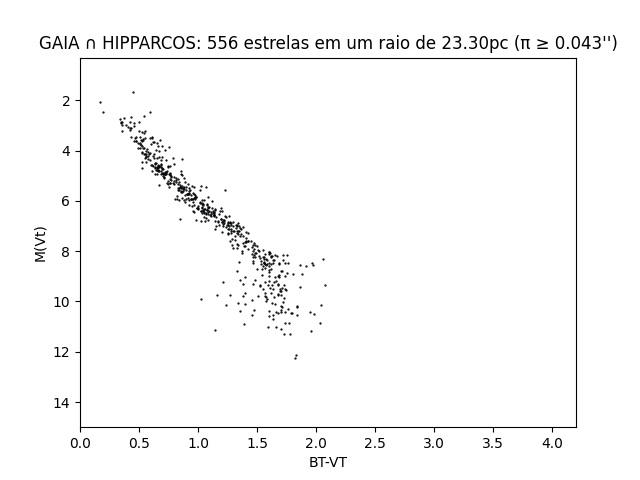
\includegraphics[width=.98\linewidth]{gaia_intersection_hipparcos_mvt_versus_bt_minus_vt_plx_greater_than_0.png}
			\captionof*{figure}{diagrama antigo}
			\columnbreak
			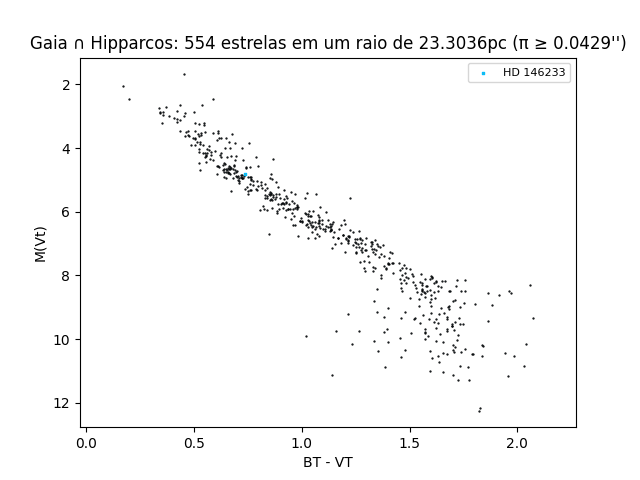
\includegraphics[width=.98\linewidth]{Gaia_intersection_Hipparcos_MVt_versus_BT_minus_VT.png}
			\captionof*{figure}{diagrama atual}
		\end{multicols}
	
		\item O diagrama \textcolor{blue}{$M(Vt)$ versus $BT-VT$} do sub catálogo Hipparcos $-$ Gaia tem $2$ estrelas a menos. O valor anterior era de $635$ estrelas, o valor correto é $633$ estrelas. 
		
		\begin{multicols}{2}
			\centering
			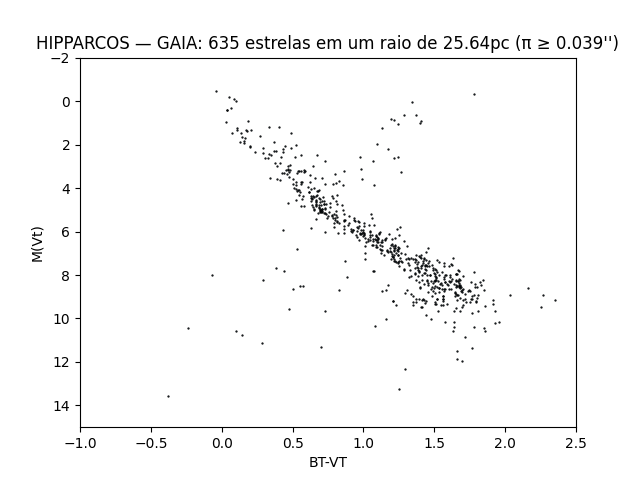
\includegraphics[width=.98\linewidth]{hipparcos_minus_gaia_mvt_versus_bt_minus_vt_plx_greater_than_or_iqual_to_0.039.png}
			\captionof*{figure}{diagrama antigo}
			\columnbreak
			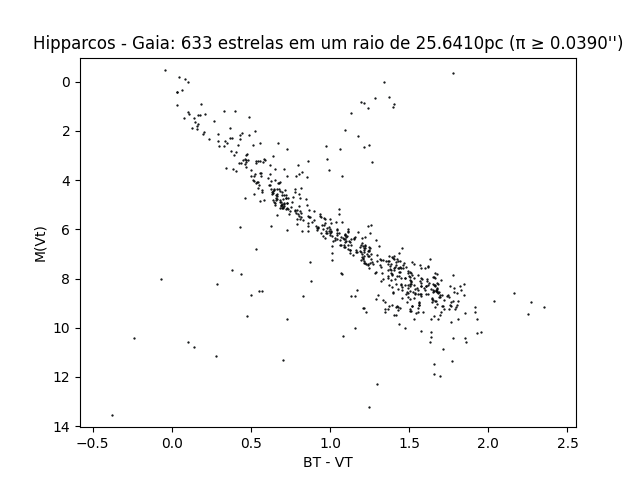
\includegraphics[width=.98\linewidth]{Hipparcos_minus_Gaia_MVt_versus_BT_minus_VT.png}
			\captionof*{figure}{diagrama atual}
		\end{multicols}
		
		\item No Diagrama \textcolor{blue}{$M(V)$ versus $B-V$} do sub catálogo Hipparcos $-$ Gaia, tem uma estrela no canto inferior direito que não estava aparecendo no diagrama anterior. Isto porque o tamanho da imagem não estava ajustado.

		\begin{multicols}{2}
			\centering
			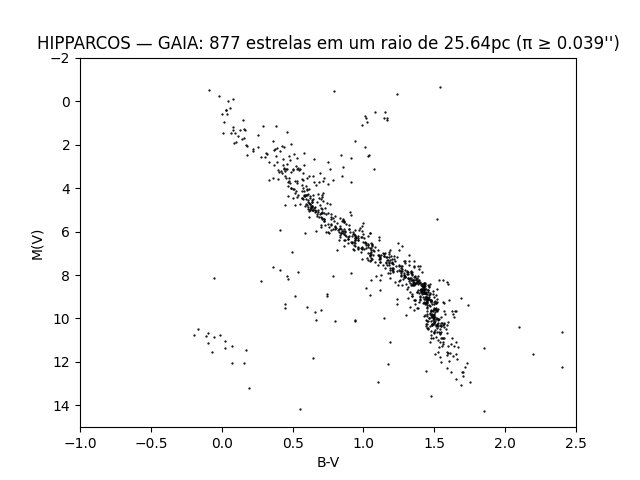
\includegraphics[width=.98\linewidth]{hipparcos_minus_gaia_mv_versus_b_minus_v_plx_greater_than_or_iqual_to_0.039.png}
			\captionof*{figure}{diagrama antigo}
			\columnbreak
			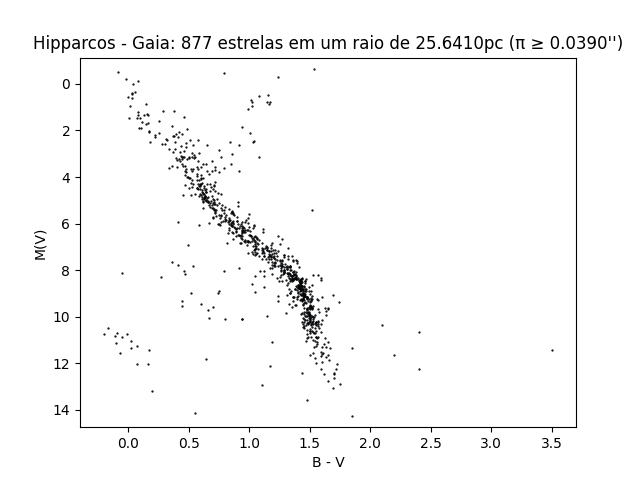
\includegraphics[width=.98\linewidth]{Hipparcos_minus_Gaia_MV_versus_B_minus_V.png}
			\captionof*{figure}{diagrama atual}
		\end{multicols}
		
		\item A quantidade de estrelas que possuem tanto designação Gaia quanto designação Hipparcos é \textcolor{blue}{$755$}. O valor anterior de $744$ foi encontrado considerando-se a distância limite de $25.64$ parsecs do catálogo $2$.
		
	    As $11$ estrelas adicionais se encaixam em alguma das seguintes situações:
		
		\begin{itemize}
			\item Possuem paralaxe no Hipparcos menor do que $0.039$\textquotesingle \textquotesingle
			\item Não possuem valor de paralaxe no Hipparcos
		\end{itemize}
	
		Abaixo, temos uma tabela com algumas informações das $11$ estrelas adicionais:

		\hspace{20pt}		

		\begin{figure}[h]
			\centering
			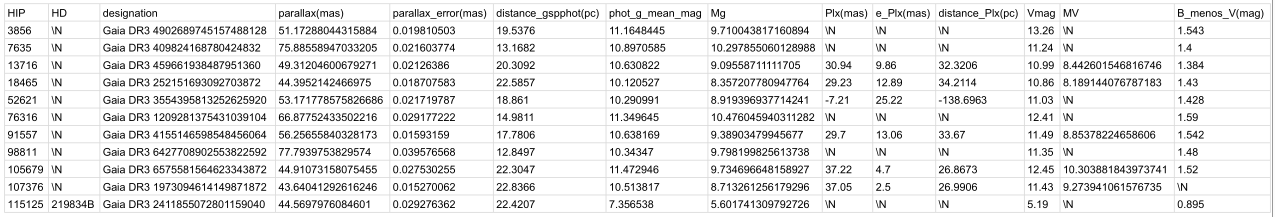
\includegraphics[width=.98\linewidth]{dados_onze_estrelas.png}
			\caption*{informações das $11$ estrelas adicionais}
		\end{figure}


		
	\end{enumerate}
	
	
\end{document}